\documentclass[border=10pt]{standalone}
\usepackage{tikz}
\usetikzlibrary{positioning, arrows.meta, fit, backgrounds, calc, decorations.pathreplacing}

\begin{document}
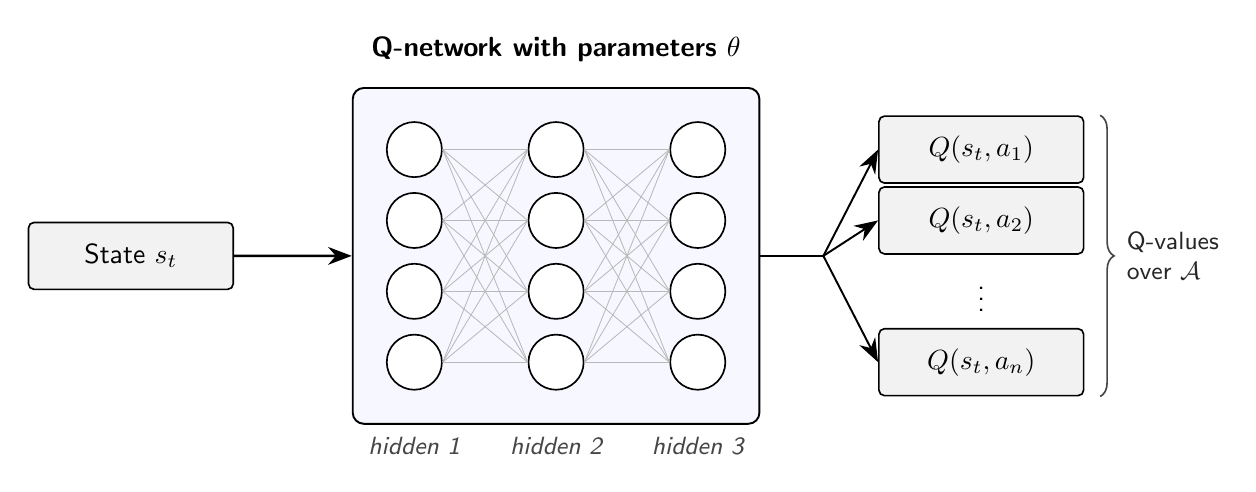
\begin{tikzpicture}[
  font=\sffamily,
  >={Stealth[length=3mm]},
  io/.style={draw, rounded corners=2pt, minimum width=2.6cm, minimum height=0.85cm, fill=gray!10, line width=0.6pt},
  neuron/.style={circle, draw, minimum size=7mm, inner sep=0pt, line width=0.6pt, fill=white},
  layerlabel/.style={font=\sffamily\small\itshape, gray!55!black},
  arrow/.style={->, line width=0.7pt},
  net/.style={draw, rounded corners=4pt, line width=0.7pt, fill=blue!3}
]

% Input — y matches the network's vertical center (mean of hidden-layer rows)
\node[io] (state) at (0, -0.3) {State $s_t$};

% Hidden layer 1 (4 neurons)
\foreach \i in {1,...,4} {
  \node[neuron] (h1-\i) at (3.6, 1.95 - 0.9*\i) {};
}
% Hidden layer 2
\foreach \i in {1,...,4} {
  \node[neuron] (h2-\i) at (5.4, 1.95 - 0.9*\i) {};
}
% Hidden layer 3
\foreach \i in {1,...,4} {
  \node[neuron] (h3-\i) at (7.2, 1.95 - 0.9*\i) {};
}

% Hidden 1 -> hidden 2
\foreach \i in {1,...,4} {
  \foreach \j in {1,...,4} {
    \draw[line width=0.3pt, gray!55] (h1-\i.east) -- (h2-\j.west);
  }
}
% Hidden 2 -> hidden 3
\foreach \i in {1,...,4} {
  \foreach \j in {1,...,4} {
    \draw[line width=0.3pt, gray!55] (h2-\i.east) -- (h3-\j.west);
  }
}

% Layer labels (placed before the box-fit so they live outside the box)
\node[layerlabel] (lbl1) at (h1-4.south) [yshift=-7mm] {hidden 1};
\node[layerlabel] (lbl2) at (h2-4.south) [yshift=-7mm] {hidden 2};
\node[layerlabel] (lbl3) at (h3-4.south) [yshift=-7mm] {hidden 3};

% Network bounding box around hidden layers only (labels sit below)
\begin{scope}[on background layer]
  \node[net, fit=(h1-1)(h1-4)(h3-1)(h3-4), inner sep=12pt] (network) {};
\end{scope}

% Network title above box
\node[font=\sffamily\bfseries, above=2mm of network] {Q-network with parameters $\theta$};

% Output Q-values
\node[io] (q1) at (10.8,  1.05) {$Q(s_t, a_1)$};
\node[io] (q2) at (10.8,  0.15) {$Q(s_t, a_2)$};
\node[draw=none, fill=none, minimum width=2.6cm, minimum height=0.85cm] (qd) at (10.8, -0.75) {$\vdots$};
\node[io] (qn) at (10.8, -1.65) {$Q(s_t, a_n)$};

% State -> network (both arrows now share the box's vertical center)
\draw[arrow, line width=0.9pt] (state.east) -- (network.west);

% Network -> outputs (single line out, then fan)
\coordinate (fan) at ($(network.east) + (0.8,0)$);
\draw[line width=0.9pt] (network.east) -- (fan);
\draw[arrow] (fan) -- (q1.west);
\draw[arrow] (fan) -- (q2.west);
\draw[arrow] (fan) -- (qn.west);

% Right brace grouping the Q outputs
\draw[decorate, decoration={brace, amplitude=5pt}, line width=0.6pt, gray!55!black]
  ($(q1.north east) + (0.20, 0)$) -- ($(qn.south east) + (0.20, 0)$)
  node[midway, right=6pt, font=\sffamily\small, gray!30!black, align=left]
  {Q-values\\ over $\mathcal{A}$};

\end{tikzpicture}
\end{document}
